\chapter{System Architecture}\label{ch:system_architechture}

\textit{Overview}
\\

The Test and Evaluation Framework (TEF) uses the information contained in a syllabus to produce a sequence of episodes for an agent learner. Figure~\ref{fig:systemlayout} depicts a high level overview of the TEF system. The syllabus passes the sequence of episodes to the TEF which sets up an environment and makes it available to the 

\begin{figure}[h]
	\centering
	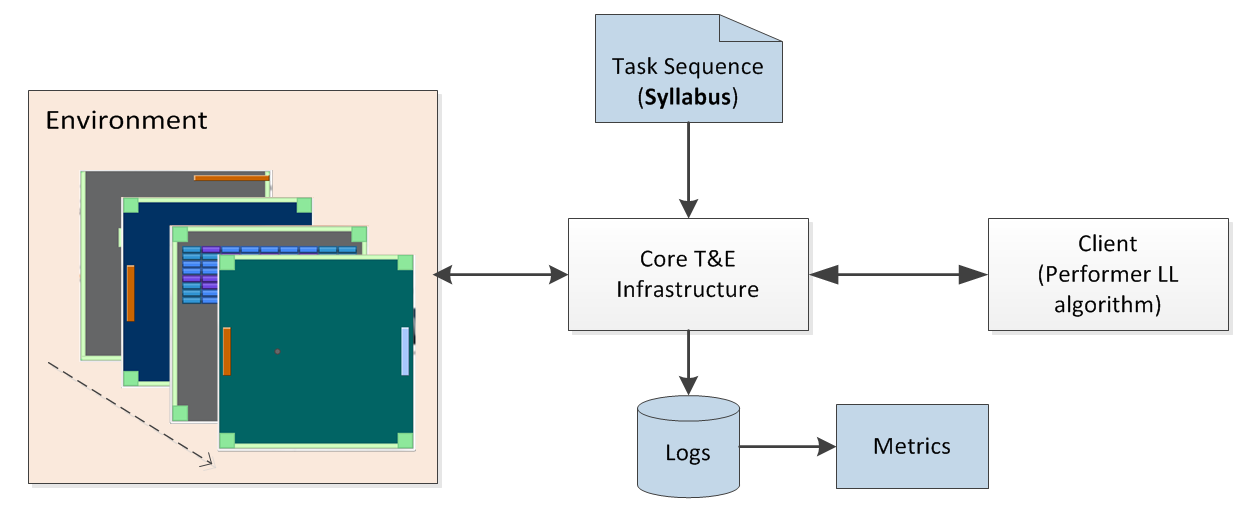
\includegraphics[width=0.85\columnwidth]{sections/figs/metrics_diagram.png}
	\caption{This figure describes the production of Metrics from Log files outputted by the Core Test and Evaluation Framework.}
	\label{fig:systemlayout}
\end{figure}

Figure~\ref{fig:syllabus} shows an example syllabus which would evaluate the Continual Learning Core Capability. You can see that only one task is exercised throughout the syllabus, but parameter variation - agent\_pos and agent\_dir are paramters for this task - is contained throughout the syllabus. Additionally, later Test phases contain previously trained parameters, allowing for a maintenance calculation. Unless otherwise noted, an instance of a syllabus is considered a Lifetime, and metrics are computed on an Agent's performance on episodes within a syllabus.

\pagebreak
\begin{figure}[h]
	\centering
	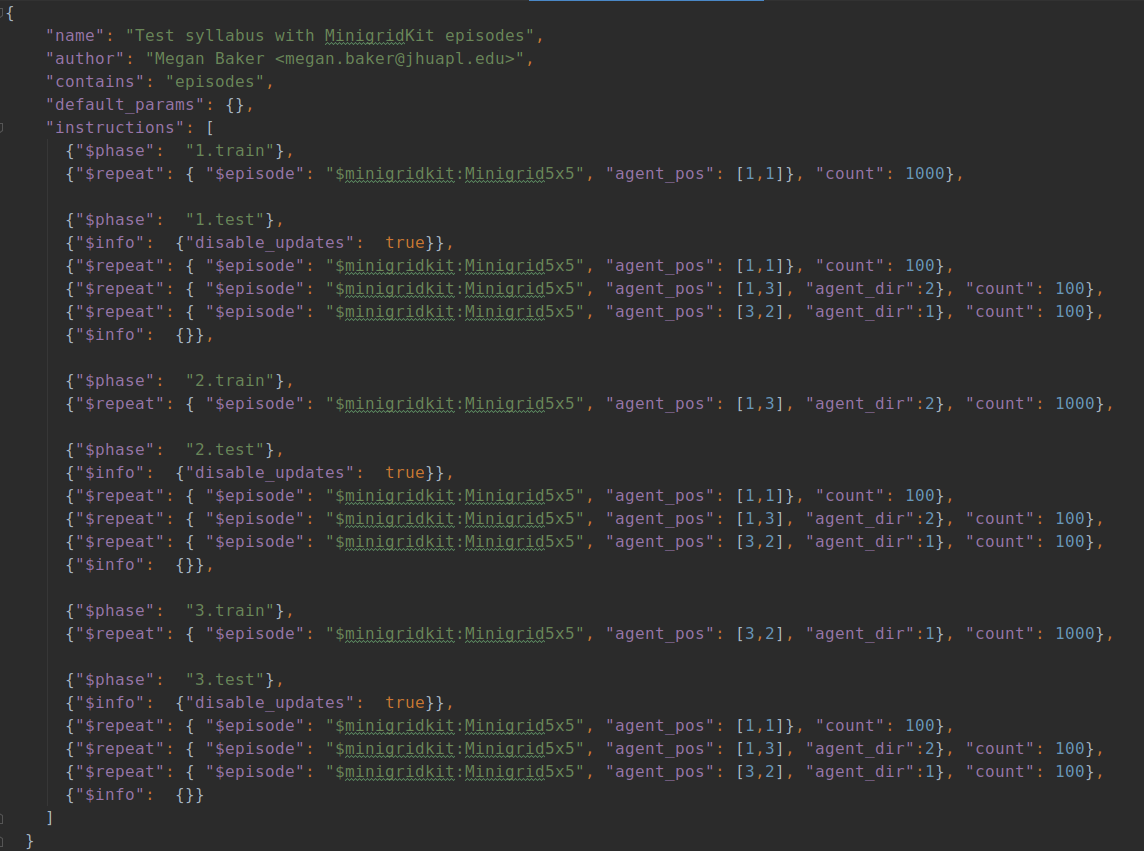
\includegraphics[width=0.75\columnwidth]{sections/figs/syllabus.png}
	\caption{An example syllabus.}
	\label{fig:syllabus}
\end{figure}



When an Agent performs episodes from the syllabus, the TEF will automatically generate logs which are saved in a tab separated file like shown in Figure~\ref{fig:logfile}. Then, the Metrics code scrapes these logs and extracts the relevant information to produce a set of scores for each metric used to evaluate the Core Capabilty being tested.\\



\begin{figure}[h]
	\centering
	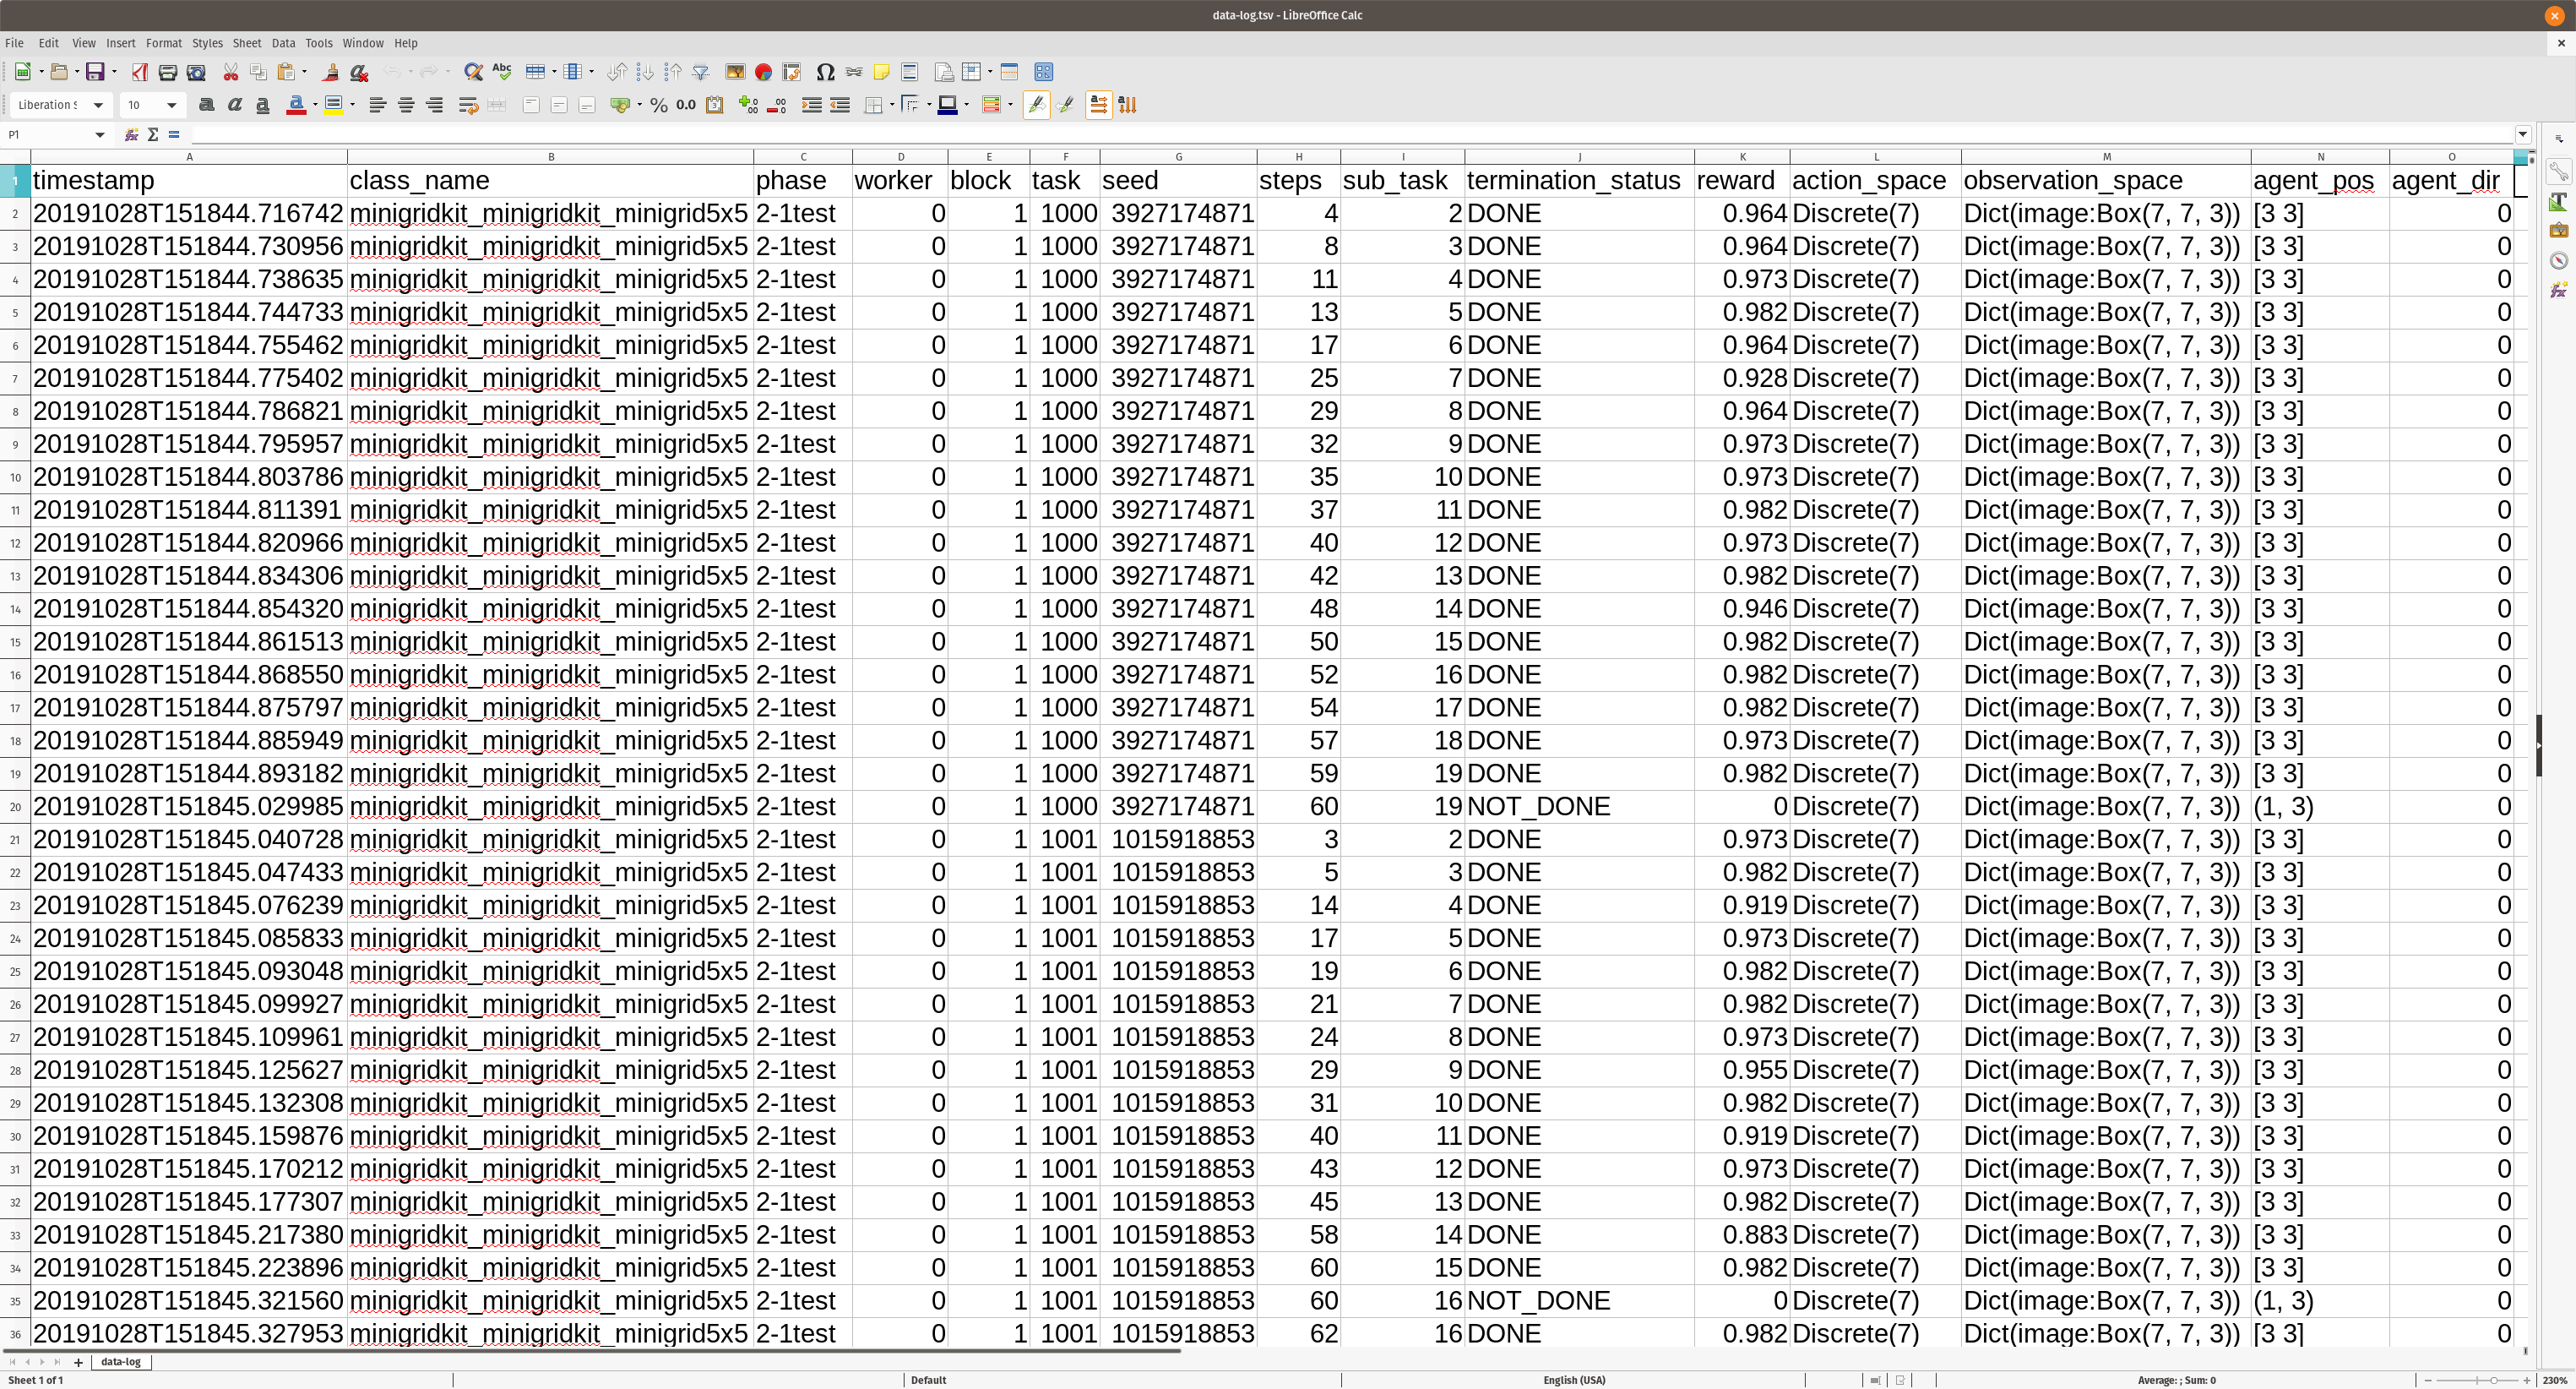
\includegraphics[width=0.75\textwidth]{sections/figs/log_file.png}
	\caption{An example log file.}
	\label{fig:logfile}
\end{figure}
